\section{\rqtwo}



Our second research question investigates the differences between program variants at runtime.
To answer RQ2, we execute each program/variant generated to answer RQ1 for \corpusrosetta corpus to collect their execution traces and execution times.
For each programs' population we compare the stack operation traces (\autoref{metric:stack}) and the execution time distributions (\autoref{metric:time}) for each program/variant pair.

This section is organized as follows. First, we analyze the programs' populations by comparing the traces for each pair of program/variant with \DTW of \autoref{metric:stack}. The pairwise comparison will hint at the results at the population level. We analyze not only the differences of a variant regarding its original program, we also compare the variants against other variants. Second, we do the same pairwise strategy for the execution time distributions \autoref{metric:time}, performing a Mann-Withney U test for each pair of program/variant times distribution. Finally, we conclude and answer RQ2.

\subsection{Stack operation traces.}


% Describe the first figure
In \autoref{rq2:dtw_distrib} we plot the distribution of all comparisons (in logarithmic scale) of all pairs of program/variant in each programs' population. All compared programs are statically different. Each vertical group of blue dots  represents all the pairwise comparison of the traces (\autoref{metric:stack}) for a program of \corpusrosetta corpus for which we generate variants.
Each dot represents a comparison between two programs' traces according to \autoref{metric:stack}. 
The programs are sorted by their number of variants in descending order. For the sake of illustration, we filter out those programs for which we generate only 2 unique variants. 

\begin{figure}[h]
    \centering
    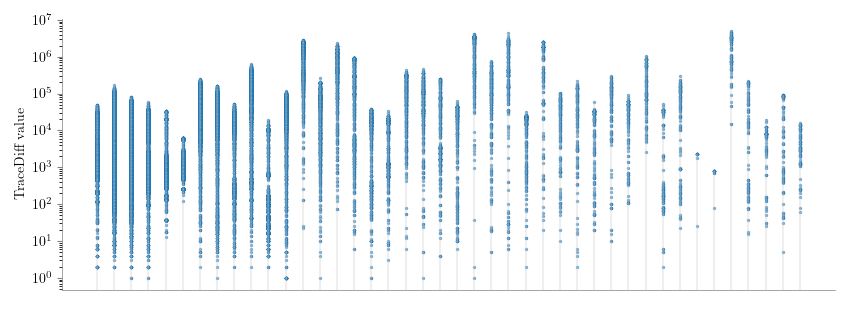
\includegraphics[width=\linewidth]{plots/plot_distribs1.png}
    \caption{Pairwise comparison of programs' population traces in logarithmic scale. Each vertical group of blue dots represents a programs' population. Each dot represents a comparison between two program execution traces according to \autoref{metric:stack}. }
    \label{rq2:dtw_distrib}
\end{figure}

% Main insight
We have observed that in the majority of the cases, the mean of the comparison values is remarkably large. We analyze the length of the traces, and one reason behind such large values of \DTW is that some variants result from constant inferring. For example, if a loop is replaced by a constant, instead of several symbols in the stack operation trace, we observe one. Consequently, the distance between two program traces is significant. 

% What happens with programs with the same trace ?
In some cases, we have observed variants that are statically different for which \DTW value is zero, \ie they result in the same stack operation trace. We identified two main reasons behind this phenomenon. First, the code transformation that generates the variant targets a non-executed or dead code. Second, some variants have two different instructions that trigger the same stack operations. For example, the code replacements below illustrate the case. 

\begin{code}[H]
\centering
\noindent\begin{minipage}{.23\linewidth}
\lstdefinestyle{nccode2}{
    numbers=none,
    firstnumber=1,
    stepnumber=1,
    numbersep=10pt,
    tabsize=4,
    showspaces=false,
    breaklines=true, 
    showstringspaces=false,
    moredelim=**[is][{\btHL[fill=black!10]}]{`}{`},
    moredelim=**[is][{\btHL[fill=celadon!40]}]{!}{!}
}
    \lstset{
        language=WAT,
        style=nccode2,
        basicstyle=\footnotesize\ttfamily,
        columns=fullflexible,
        breaklines=true
    }
    \begin{lstlisting}
(1) `i32.lt_u`
(2) `i32.le_s`
    \end{lstlisting}
\end{minipage}\hfill%
\noindent\begin{minipage}{0.2\linewidth}
\lstdefinestyle{nccode2}{
    numbers=none,
    firstnumber=1,
    stepnumber=1,
    numbersep=10pt,
    tabsize=4,
    showspaces=false,
    breaklines=true, 
    showstringspaces=false,
    moredelim=**[is][{\btHL[fill=black!10]}]{`}{`},
    moredelim=**[is][{\btHL[fill=celadon!40]}]{!}{!}
}

    \lstset{
        language=WAT,
        style=nccode2,
        basicstyle=\footnotesize\ttfamily,
        columns=fullflexible,
        breaklines=true
    }
    \begin{lstlisting}
!i32.lt_s!
!i32.lt_u!
    \end{lstlisting}
\end{minipage}\hfill%
\noindent\begin{minipage}{.3\linewidth}
\lstdefinestyle{nccode2}{
    numbers=none,
    firstnumber=1,
    stepnumber=1,
    numbersep=10pt,
    tabsize=4,
    showspaces=false,
    breaklines=true, 
    showstringspaces=false,
    moredelim=**[is][{\btHL[fill=black!10]}]{`}{`},
    moredelim=**[is][{\btHL[fill=celadon!40]}]{!}{!}
}

    \lstset{
        language=WAT,
        style=nccode2,
        basicstyle=\footnotesize\ttfamily,
        columns=fullflexible,
        breaklines=true
    }
    \begin{lstlisting}
(3) `i32.ne`
(4) `local.get 6`
    \end{lstlisting}
\end{minipage}\hfill%
\noindent\begin{minipage}{0.2\linewidth}
\lstdefinestyle{nccode2}{
    numbers=none,
    firstnumber=1,
    stepnumber=1,
    numbersep=10pt,
    tabsize=4,
    showspaces=false,
    breaklines=true, 
    showstringspaces=false,
    moredelim=**[is][{\btHL[fill=black!10]}]{`}{`},
    moredelim=**[is][{\btHL[fill=celadon!40]}]{!}{!}
}

    \lstset{
        language=WAT,
        style=nccode2,
        basicstyle=\footnotesize\ttfamily,
        columns=fullflexible,
        breaklines=true
    }
    \begin{lstlisting}
!i32.lt_u!
!local.get 4!
    \end{lstlisting}
\end{minipage}
\end{code}

In the four cases, the operators are different (original in gray color and the replacement in green color) leaving the same values for equal operands.
The (1) and (2) cases are comparison operations leaving the value $0$ or $1$ in the stack taking into account the sign of their operands.  In the third case, the replacement is less restricted to the original operator, but in both cases, the codes leave the same value in the stack. In the last case, both operands load a value of a local variable in the stack, the index of the local variable is different but the value of the variable that is appended to the trace is the same in both cases. 

\subsection{Execution times.}

%\todo{recall again that execution time diversification is important, should the reader have forgotten about this.}

Even when two programs of the same population offer different execution traces, their execution times can be similar (statistically speaking). In practice, the execution traces of \wasm programs are not necessarily accessible, being not the case with the execution time. For example, in our current experimentation we need to use our own instrumentation of the execution engine to collect the stack trace operations while the execution time is naturally accessible in any execution environment. This mentioned reasoning enforces our comparison of the execution times for the generated variants. Besides the execution times of programs can be used by malicious clients to construct personalized attacks \cite{morgan2015web}. Therefore, by measuring the execution times, we assess the diversification of observable behaviors evaluated in real-world security scenarios.


For each program's population, we compare the execution time distributions, \autoref{metric:time}, of each pair of program/variant.
Overall diversified programs, $169$ out of $239$ ($71\%$) have at least one variant with a different execution time distribution than the original program (P-value $<$ $0.01$ in the Mann-Withney test). This result shows that we effectively generate variants that yield significantly different execution times.

By analyzing the data, we observe the following trends. First, if our tool infers control-flows as constants in the original program, the variants execute faster than the original, sometimes by one order of magnitude. On the other hand, if the code is augmented with more instructions, the variants tend to run slower than the original. 

In both cases, we generate a variant with a different execution time than the original. Both cases are good from a randomization perspective since this minimizes the certainty a malicious user can have about the program's behavior. Therefore, a deeper analysis of how this phenomenon can be used to enforce security will be discussed in answering RQ3.

To better illustrate the differences between executions times in the variants, we dissect the execution time distributions for one programs' population of \corpusrosetta. The plots in \autoref{rq3:perf} show the execution time distributions for the \texttt{Hilbert curve} program and their variants. 
We illustrate time diversification with this program because, we generate unique variants with all types of transformations previously discussed in \autoref{results:rq1}.
In the plots along the X-axis, each vertical set of points represents the distribution of 100000 execution times per program/variant. The Y-axis represents the execution time value in milliseconds. The original program is highlighted in green color: the distribution of 10000 execution times is given on the left-most part of the plot, and its median execution time is represented as a horizontal dashed line. The median execution time is represented as a blue dot for each execution time distribution, and the vertical gray lines represent the entire distribution. The bolder gray line represents the 75\% interquartile. The program variants are sorted concerning the median execution time in descending order.

\begin{figure*}[h]
    \centering
    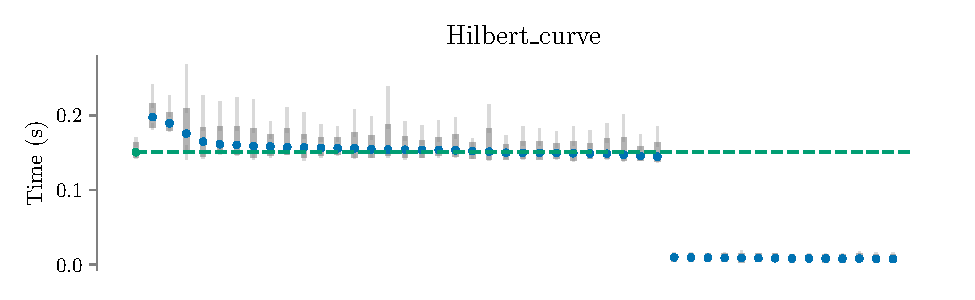
\includegraphics[width=\linewidth]{plots/hilbert_curve.pdf}
    \caption{Execution time distributions for \texttt{Hilber\_curve} program and its variants. Baseline execution time mean is highlighted with the magenta horizontal line. }
    \label{rq3:perf}
\end{figure*}

% explanation
For the illustrated program, many diversified variants are optimizations (blue dots below the green bar). The plot is graphically clear, and the last third represents faster variants resulting from code transformations that optimize the original program.
Our tool provides program variants in the whole spectrum of time executions, lower and faster variants than the original program. The developer is in charge of deciding between taking all variants or only the ones providing the same or less execution time for the sake of performance. Nevertheless, this result calls for using this timing spectrum phenomenon to provide binaries with unpredictable execution times by combining variants. The feasibility of this idea will be discussed in \autoref{results:rq3}.


\begin{tcolorbox}[title=Answer to RQ2.,boxrule=2pt,arc=.3em,boxsep=1.5mm]
    We empirically demonstrate that our approach generates program variants for which execution traces are different. We stress the importance of complementing static and dynamic studies of programs variants. For example, if two programs are statically different, that does not necessarily mean different runtime behavior. There is at least one generated variant for all executed programs that provides a different execution trace. 
    % answer to RQ2
    We generate variants that exhibit a significant diversity of execution times. Concretely, for $169/239\,(71\%)$ of the diversified programs, at least one variant has an execution time distribution that is different compared to the execution time distribution of the original program. 
    The result from this study encourages the composition of the variants to provide a resilient execution.
\end{tcolorbox}